\documentclass{article}
\usepackage{graphicx}
\usepackage[fontsize=11pt]{scrextend}
\title{PowerEnjoy Service - Design Document}
\begin{document}

\begin{titlepage}
\begin{figure}
	\centering
	\includegraphics{polimi}
\end{figure}
\maketitle
\centering
Prof. Luca Mottola
\newline
\raggedleft
Authors:
\begin{itemize}
	\raggedleft
	\item ZHOU YINAN(Mat. 872686)
	\item ZHAO KAIXIN(Mat. 875464)
	\item ZHAN YUAN(Mat. 806508)	
\end{itemize}
\end{titlepage}

\tableofcontents
\newpage

	
	\section{INTRODUCTION}
	\subsection{Purpose}
	The Design Document serves to describe the structure of the PowerEnJoy service. It provides all the detailed information for building the system. More precisely, it provides the information on the chosen architecture style and design pattern. It explains how the components are implemented and interacted in the system. The document also provides the verification of fulfilling the requirements listed in the RASD documents. In general, the document is served as a guideline for program developers.
	\subsection{Scope}
	The Design Document shows how the system is built and explains how the functional requirements in the RASD file are realized. The document covers high level architecture design, interacting components,  algorithms and user interface design. 
	\subsection{Definitions, Acronyms, Abbreviations}
	\begin{itemize}
		\item RASD : Requirement Analysis and Specification Document
		\item DD : Design Document
		\item MVC : Model View Controller
		\item REST : Representational state transfer (REST) or RESTful web services are one way of providing interoperability between computer systems on the Internet.
		\item JSON : JSON (JavaScript Object Notation) is a minimal, readable format for structuring data. 
	\end{itemize}
	\subsection{Reference Documents}
	\begin{itemize}
		\item Specification Document Assignments AA 2016-2017
		\item RASD
	\end{itemize}
	\newpage
	\subsection{Document Structure}
	The Design Document is divided into 7 parts : 
	\begin{itemize}
		\item \textbf{Introduction} : This section introduces the structure of Design Document and some basic background knowledge to understand the document.
		\item \textbf{Architecture Design}
		\\1. High level components and their interactions : This section gives a general description of how the components are defined and how they communicate with each other  
		\\2. Component view : This section gives detailed information of components defined in the system
		\\3. Deployment view : This section describes how the components are deployed in order to act correctly
		\\4. Runtime view : This section gives the sequential diagrams of how the users accomplish their requests
		\\5. Component interfaces : The interfaces of components are described in this section
		\\6. Selected architectural styles and patterns : This section explains the reason of choosing certain architecture and the benefits accompanied
		\\7. Other design decisions
		\item \textbf{Algorithm Design} : In the section, the necessary code samples are given in order to clearly demonstrate the component interaction 
		\item \textbf{User Interface Design} : this section presents the user interface 
		\item \textbf{Requirement Traceability} : This section shows how the requirements in the RASD are accomplished in the design
	\end{itemize}
	\newpage
	\section{ARCHITECTURAL DESIGN}
	
	\subsection{High level components and their interaction}
	\begin{figure}[h]
	\includegraphics[width=\textwidth]{high}
	\end{figure}
	Here we choose to use the 3 tier architecture: The Presentation tier includes the Client Mobile Application, Client Web Browser and the Car Application; The Business tier includes the Server; The Data tier includes the database.
	\\
	\\Here a MVC pattern is also used. The presentation tier is responsible for all the GUI part, thus it is the view part. The server maintains all the business logic and the database is responsible for data manipulation. Thus the model and controller are in the server and database side. 
	\newpage
	
	\subsection{Component view}
	\begin{figure}[h]
	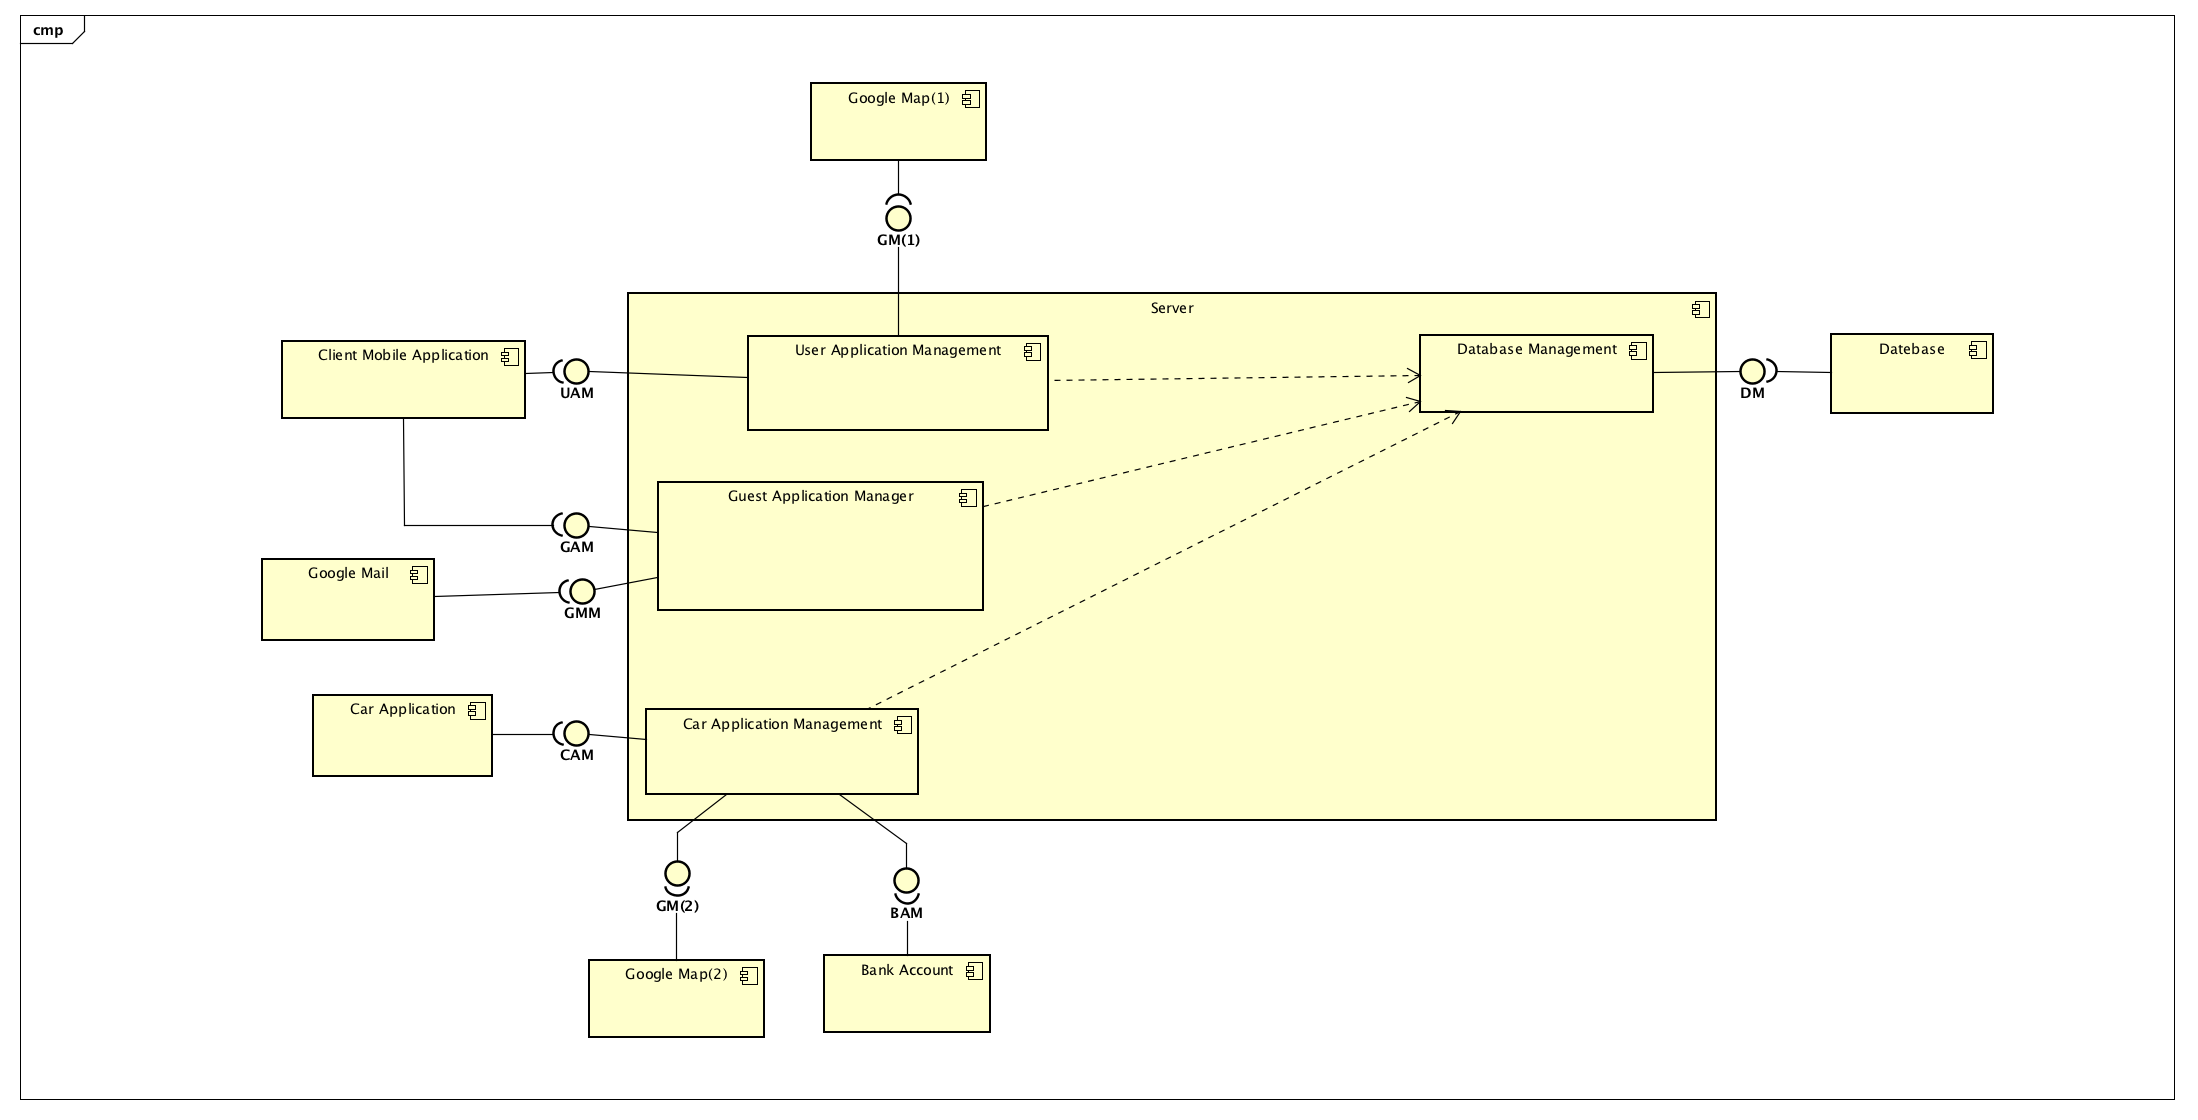
\includegraphics[width=\textwidth]{CV_Server}
	\end{figure}
	For the Server, there should be several interfaces, which are in charge of communicating with other components: 
	\begin{itemize}
		\item \textbf{User Application Manager} : Component that provides the interface for the users of the system and the Google Map. User Application Manager should provide the options of checking the available cars around the specified position, reserving car and canceling the reservation. With the help of the Google Map, the system can know the location of the user.
		\item \textbf{Guest Application Manager} : Component that provides the interfaces for the unregistered guest of the system and the Google Mail. It provides the option to create an account. Finishing the register, the system would send an e-mail to the guest through the Google Mail.
		\item \textbf{Car Application Manager} : Component that provides the interface for the car Application, Google Map and Bank Account. The Car Application Manager can know the location of the car, charge the specified bank account and send the instructions to the car.
		\item \textbf{Database Manager} : Component that provides the interface for the Database for collecting the information provided by other components.   
	\end{itemize}
	\newpage
	\begin{figure}[h]
	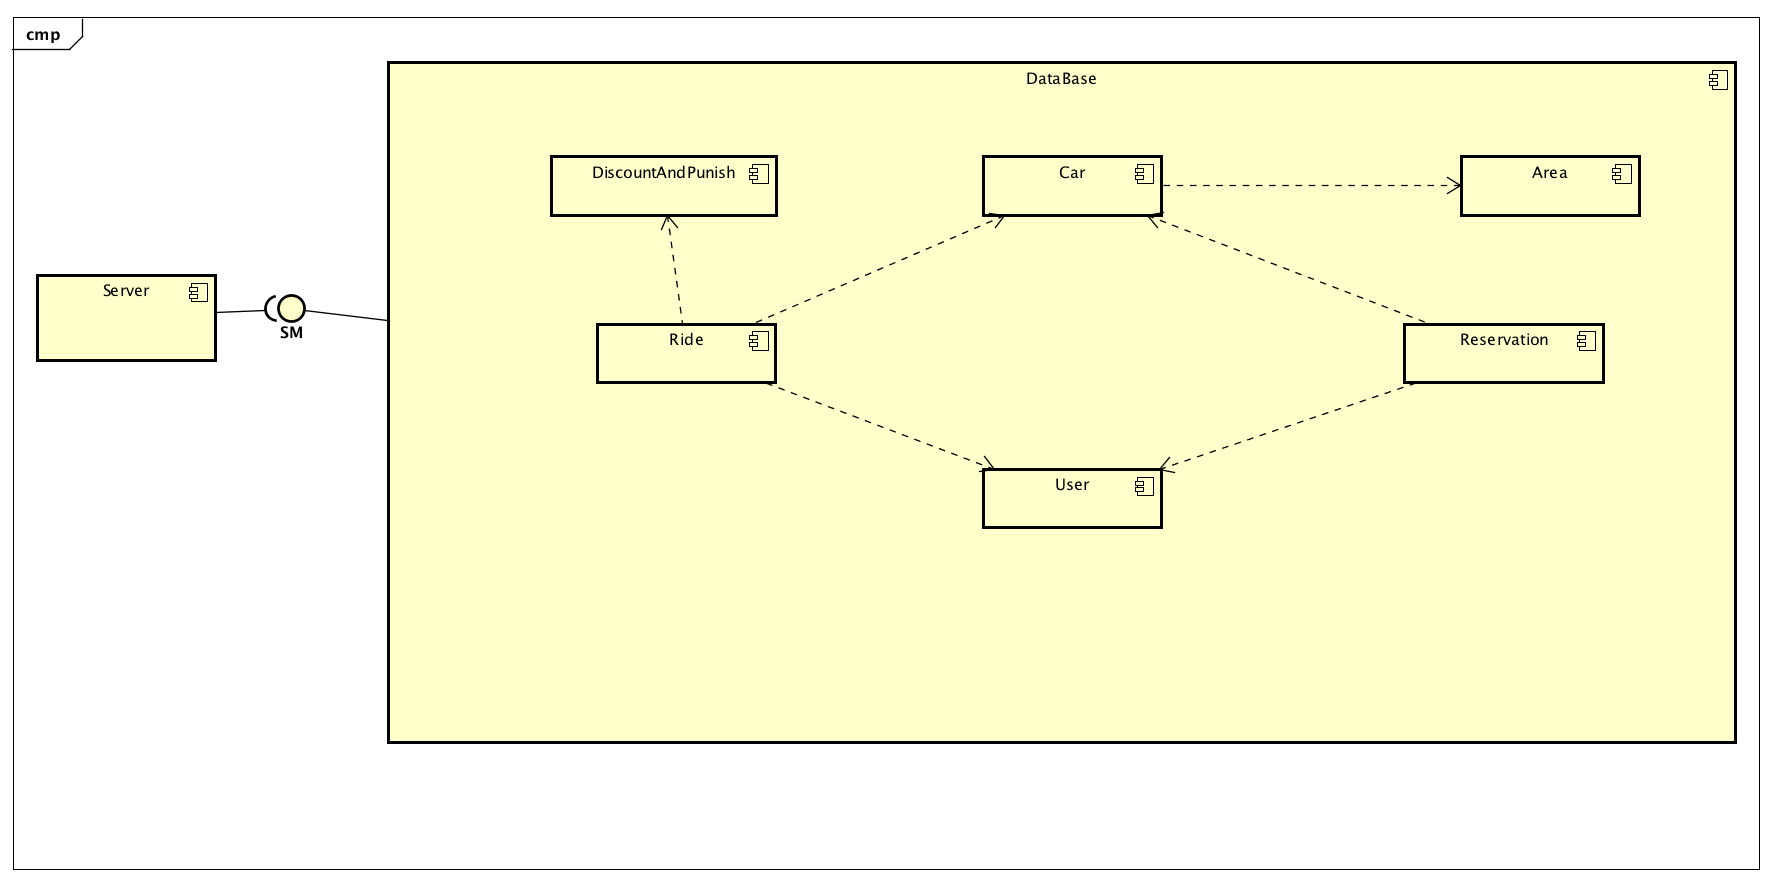
\includegraphics[width=\textwidth]{CV_Database}
	\end{figure}
	For the Database, there are several components for storing the data of the system. The Database should provide the interface of the Server for information exchange. Through the interface, the Server can transmit and  store the information in the Database. The Server can also retrieve the information from the Database according to the corresponding instruction.

	\begin{itemize}
		\item \textbf{Car} : Component that stores the information of the cars. The Car should store the position, plate, battery, capacity, state and the currentPosition of each car.
		\item \textbf{User} : Component that stores the information of the users. The User should stores the credential and the paymentInfo of each user.
		\item \textbf{Ride} : Component that stores the information of the riding. The Ride should store the riding information, including the renting car, corresponding user and so on.
		\item \textbf{Reservation} : Component that stores the information of the reservation. The Reservation should store the user and the corresponding car of each reservation.
		\item \textbf{DiscountAndPunish} : Component that stores the information of the discount and punishment of each ride. For each ride, when finishing the riding, the DiscountAndPunish component should provide the information about the discount and the punishment info for calculating the total charge.
		\item \textbf{Area} : Component that stores the area of each position.
	\end{itemize}
	\newpage

	\subsection{Deployment view}
	\begin{figure}[h]
		\includegraphics[width=\textwidth]{Deployment}
	\end{figure}
	\newpage
	\subsection{Runtime view}
	\subsubsection{Register}
	\begin{figure}[h]
		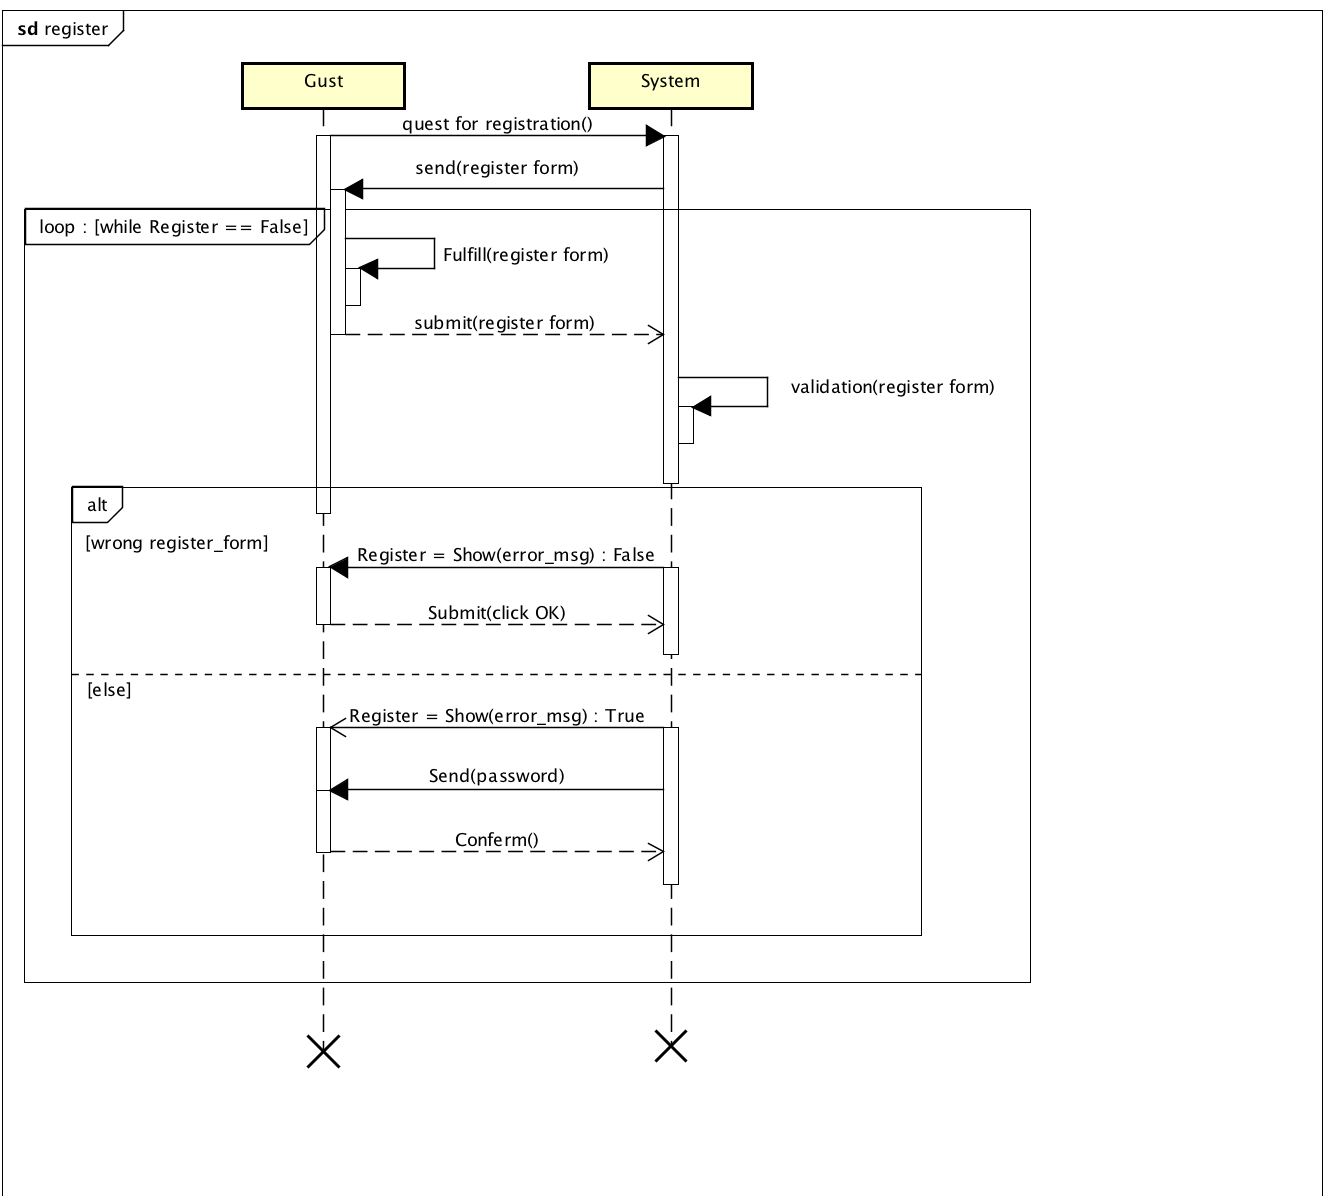
\includegraphics[width=\textwidth]{register}
	\end{figure}
	The sequence diagram shows procedure of registration. It starts when a guest requests the registration on the client application. After guest fulfilling the register form , the information will be sent to the server, where guest application manager checks for validation. It accesses, through the database manager, the database and checks if the information already exists. In the negative case, the server sends back to application interface a message with error; in the affirmative case,the server allows the database to memorize the guest's credential and password, and Guest Application Manager will send back an email to guest with Password created.   
	
	\newpage
	\subsubsection{Login}
	\begin{figure}[h]
		\includegraphics[width=\textwidth]{Login}
	\end{figure}
	This sequence diagram shows the procedure of users  logging into the system. The Client Application sends to the server  the user's email and password to check for correctness.If a corresponding tuple exists in the data base, the Guest Application Manager sends back the user information in the format of JSON;If not, the server sends to client application an error message.
	\newpage
	\subsubsection{Reserve}
	\begin{figure}[h]
		\includegraphics[width=\textwidth]{reserve}
	\end{figure}
	This sequence diagram shows how a user can reserve a car. First the user inserts a position where he wants to start the ride,it can either be inserted by user or generated by GPS automatically. This information will be sent to User Application Manager, it gets all the car information form data base and selects certain cars within nearby distance. Then the list of cars will be sent back. And the Client  application, after user confirming the selection,notifies the User Manager. The User Manager then  calls Database Manager to insert into the database the reservation information. Finally a message will be sent to application, notifying the user the successful reservation.\\
	\\The reservation lasts for one hour. At the end of this time, the reservation will be canceled. the server updates the reservation state, changes the car state into Free,charges 1EUR , and at last sends an email to notify the user the cancellation and punishment fee.
	
	\subsubsection{Pick up}
	\begin{figure}[h]
		\includegraphics[width=\textwidth]{openDoor}
	\end{figure}
	When the user is near the car, he sends his current location to notice the server. Car Manager then verifies whether the position received is  near enough to unlock the car. It sends back a message with positive or negative confirmation based on the result of verification. Moreover  Car Manager sends a command to the corresponding car in order to unlock it.
	
	\newpage

	\subsubsection{Renting}
	\begin{figure}[h]
		\includegraphics[width=\textwidth]{rent}
	\end{figure}
	\newpage
	The sequence  shows how to start a ride.  User can optionally  choose to enable money save option or not. After Ignition of the car engine, there are some sensors in the car that can detect how many passengers are there.  If it's more than 2 people (exclude user), the Car Manager will apply 10 percent of discount on this ride. During the ride a display shows the information(time ,cost) of the journey. There are some other conditions for discount based on the state of car after the ride. The server checks which one is presented and applies the corresponding discount. The total price will be calculated by Car Manager and sends back to Client application.

	\subsection{Component interfaces}
	\begin{figure}[h]
		\includegraphics[width=\textwidth]{interface}
	\end{figure}
	\subsubsection{Client app}
	\textbf{register(name, surname, email,drivingLisence,paymentInfo)}
	\\
	\\The register function on the Client app side receives from input all the necessary information for registering. This information is then sent to the server in the format of JSON for former processing.
	\\
	\\\textbf{logIn(email, password)}
	\\
	\\The logIn function receives from the input the user's email and corresponding password. This information is then sent to the server in the format of JSON for former processing. 
	\\
	\\\textbf{car[] getAvailableCars(location)}
	\\
	\\By providing a location, users can get all the available cars nearby. The location information is sent to the server in the format of JSON then the server sends back all the cars that are available near that location. 
	\\
	\\\textbf{void reserve(user, car)}
	\\
	\\The reserve function allows a user to reserve a car. The reserve request is then sent to the reservation Manager in the server.
	\\
	\\\textbf{void openTheDoor(car,location)}
	\\
	\\When the user gets to the reserved car, he can inform the server that he is nearby by sending his current location to the server. 
	
	\subsubsection{Car app}
	\textbf{void startRide(user, car)}
	\\
	\\Car app notifies the server that a ride starts.
	\\
	\\\textbf{void endRide(user, car, state)}
	\\
	\\Car app notifies the server that a ride is finished.
	\\
	\\\textbf{String getCurrentPrice(user,car)}
	\\
	\\The working car can get the current price information from the server.
	\subsubsection{Guset Manager}
	\textbf{Boolean register(credentials)}
	\\
	\\The register function receives from clients the credentials. The Guest Manager in the server checks whether the received credentials already exist in the database or not. In the case of new coming credentials, the Guest Manager uses Gmail API to send an email to the guest with a newly generated password. Then Guest Manager creates a new tuple using credentials and password and inserts it into the database. In the case of a successful register, a true value will be sent to the cilent app.  In the case of non valid credentials, the server sends back a false notation to the client app.
	\\
	\\\textbf{String signIn(email, password)}
	\\
	\\The signIn function checks the email and password provided by the user in the server side. If they are valid i.e. there exists a corresponding email and the password matches the email, then the information of the user will be encoded into a JSON format and be sent back to the client app. 
	
	\subsubsection{User Manager}
	\textbf{String reserver(user, car)}
	\\
	\\User makes request to the server for a car reservation. User Manager processes the request and makes reservation to the corresponding car.  The reservation information is then stored into database and the corresponding car information will be sent back to client app in the format of JSON.
	\\
	\\\textbf{Boolean reservationTimeOut(user, car)}
	\\
	\\When the reserved car is timing out, User Manager notifies the corresponding user and cancels the reservation.
	
	\subsubsection{Car Manager}
	\textbf{Ride startRide(user,car)}
	\\
	\\Car Manager on the server side receives from car app the user and car information. It checks from the database whether the ride request is valid or not. In the case of a valid request, server sends back to the client app a successful notation. Also Car Manager stores the data into the database. In the case of a non-valid request, the server sends back to the car app an error notation.
	\\
	\\\textbf{String endRide(user,car,state)}
	\\
	\\Car Manager processes the request of ending a ride from the car app. It gets the ride information from the database and calculates the final price of the ride. Then Car Manager sends back to car app the price  needs to pay. Car Manager redirects payment request to the bank service. 
	\subsection{Selected architectural styles and patterns}
	\subsubsection{Architecture}
	We choose the three-tier architecture for our system. The whole system is divided into three parts : presentation tier, business tier and data tier.
	\begin{itemize}
		\item presentation tier : It contains Client app and Car app. It is the layer that directly interacts with the actors. 
		\item business tier : Business tier contains all the logic. It manages request and response. Also it manages the data interaction with the database. By using the business tier, clients do not directly interact with the database. 
		\item data tier : We use MySQL database to store all the useful data.
	\end{itemize}
	\begin{figure}[h]
	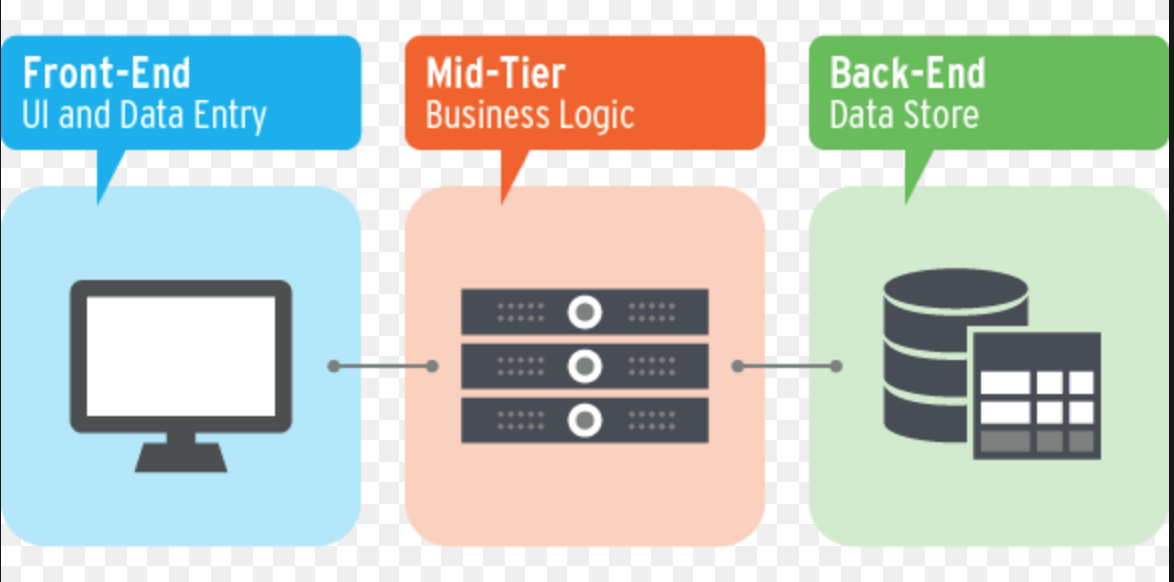
\includegraphics[width=\textwidth]{architecture}
	\end{figure}
	The three tier architecture is used because an effective distributed client-server design is needed. It guarantees increased performance, flexibility, maintainability, reusability, and scalability, while hiding the complexity of distributed processing from the user. In our system, no direct database access from the client app is allowed. All the requests are passing through business tier first.
	\\
	\\We use a typical client-server architecture. In the client-server architecture, data is manipulated in the server side and can only be accessible to designated users. Moreover, services can be easily maintained or updated in the server side without touching Client app.
	\\
	\\The Client app is composed of a mobile application and a web browser. Users can choose to access the service by either a mobile web browser or an application. Our system uses request-response methodology. All the services are requested from the user side. The client asks for information or requests for certain services using REST and server responses in JSON format. When the server receives a certain request, it dispatches the request to corresponding responsible manager. 
	\\
	\\We use RESTFUL API for for our service to be processed. Each service is defined by a unique URI. By using RESTFUL API, we keep our client-server communication clear and simple. Moreover, REST style client-server architecture allows stateless session in the server. All the information transfered between server and client side is in JSON format which allows the information to be processed by different end-systems. 
	\subsubsection{Pattern}
	\textbf{MVC} Model-View-Controller is used in our system. To combine it with our three-tier architecture, the view part lies on the client app side which deals with interaction with users. Model and Controller are in the server side, which maintains business logic and manipulation of data. 
	\\
	\\\textbf{Client-Server} In our system, there are 2 clients: user application and car application. The user application can be a pure iOS or Android app or it can be a mobile web browser. In both cases, we use RESTFUL API to communicate with the server. The information sent and received is in JSON format.
	\\
	\\\textbf{Request-response} Our system is based on service which uses request-response methodology. All the requests are generated from the user side which can be either a user application or a cat application. Server is responsible for processing the request and sending back the response.
	
	\subsection{Other design decisions}
	The main design architecture and patterns are described above. Just to mention, our system uses some other service api to meet the requirements. For example, we use Google map api to deal with geographical information. Also all the billing requests are forwarded to other bank payment systems.  
	\newpage
	\section{ALGORITHM DESIGN}
	In out system, we have not used any complex algorithms. The request-response methodology is pretty straight forward. In this section, some important interface functions  are described in pesudocode.
	\begin{verbatim}
	function dispatch(String request) {
	
		String url = parse(request);
	
		switch(url) {
	
			case "register" : forwardTo(Gust Manager);	
			case "logIn" : forwardTo(Guest Manager);	
			case "reserve" : forwardTo(User Manager);	
			case "openTheDoor" : forwardTo(User Manager);	
			case "startRide" : ForwardTo(Car Manager);
			case "endRide" : ForwardTo(Cae Manager); 
		}
	}
	
	function calculateDistance(Position x1, Postion x2}) {
		
		//using Googla Map api to calcualte distance
		
		lag1 = x1.latitude;
		lon1 = x1.longitude;
		lag2 = x2.latitude;
		lon2 = x2.latitude;
		distance = calculate(lag1,lon1,lag2,lon2);
	}
	
	function getAvailableCars(Position location) {
		
		Map carDistance = new HashMap();
		for all car in Cars {
			if ()dis = distance(car.position, location)) < nearbyDistance 
				carDistance.add(car,dis);
		}
		return car.Distance.sortedByDistance()
	}
	
	
	\end{verbatim}
	
	\section{USER INTERFACE DESIGN}
	This section will describe different interfaces for the components. Component interfaces are divided into three different aspects : Guest Manager, User Manager and Car Manager.
	\subsection{HomePage,Registration,Login}
	\begin{figure}[!htb]
		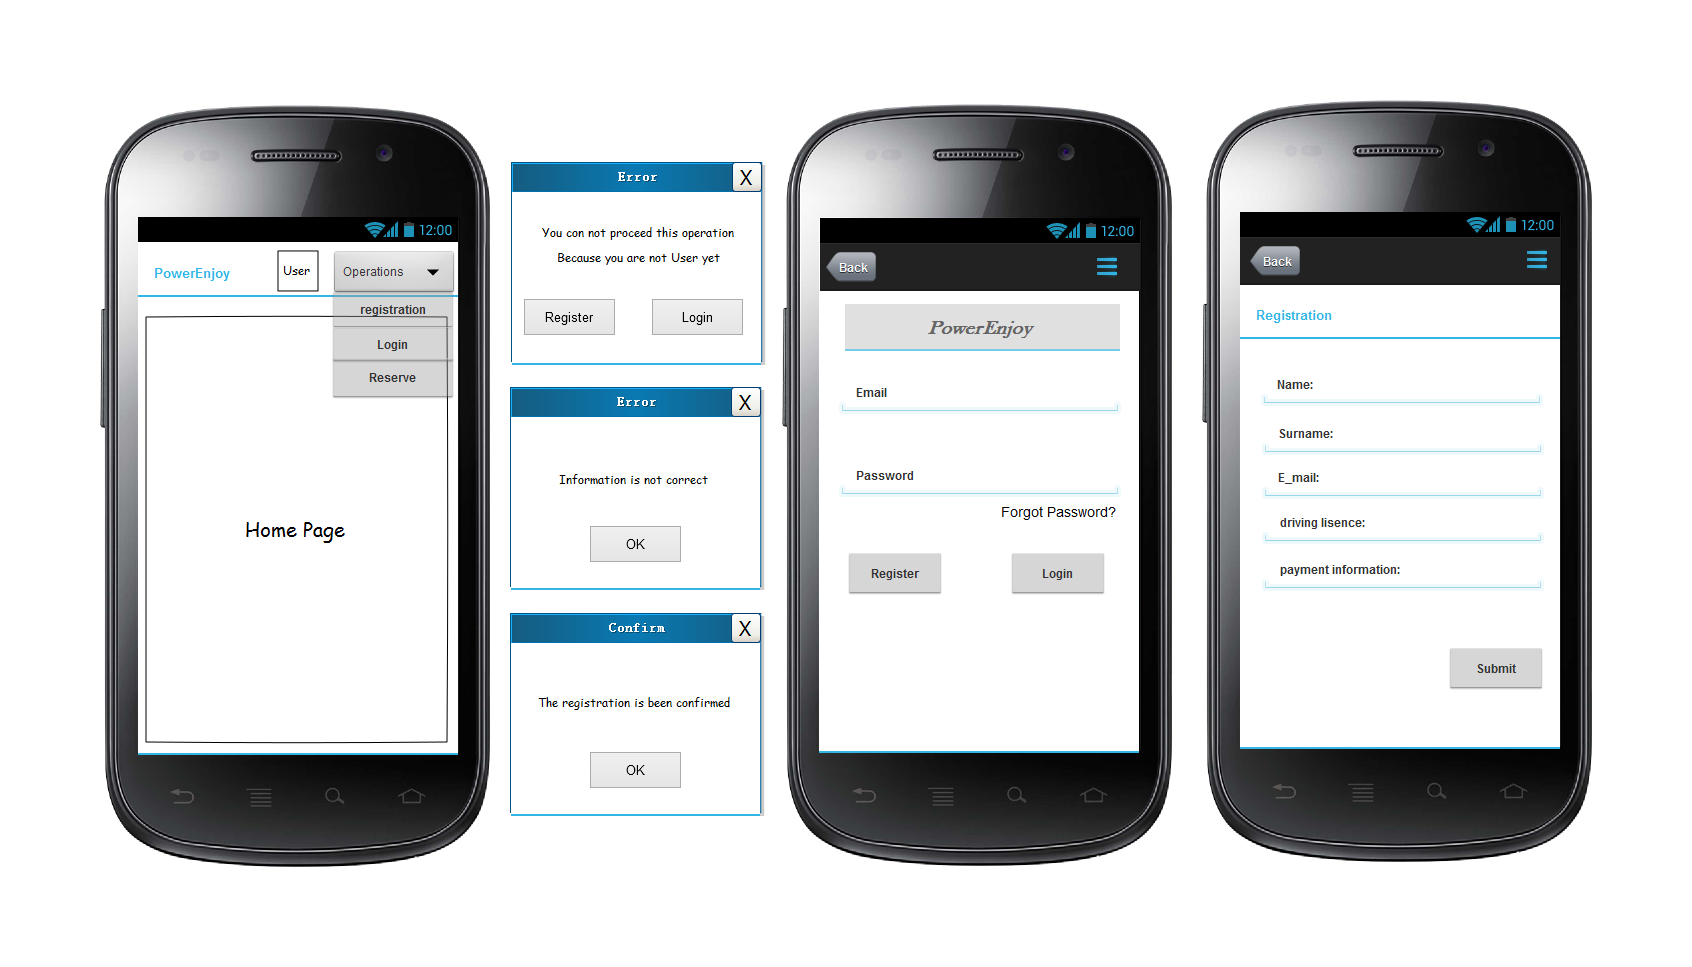
\includegraphics[width=\textwidth]{HomePage,Registration,Login} 
	\end{figure}
	In the HomePage(leftmost one) there is a menu list which contains the operation that users can do(registration, register,login).If a guest press the reservation, a window appear to notify guest to register or login. Other two interfaces are respectively Login and Register interface. After the submit, based on the result, it will open a pop-up window to notify the user.
	\newpage
	\subsection{Registration,Pick up}
	\begin{figure}[h]
		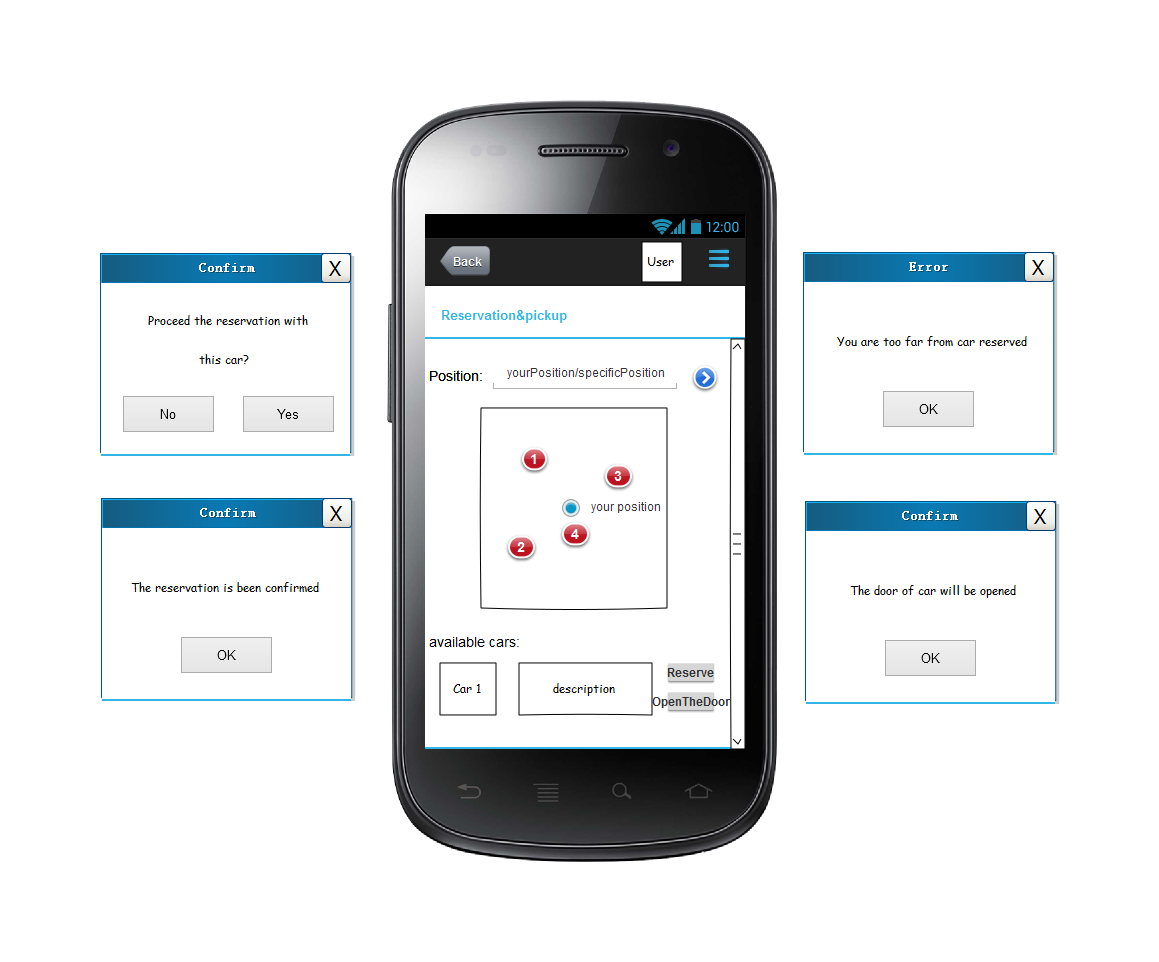
\includegraphics[width=\textwidth]{Reservation,PickUp} 
	\end{figure}
	In this page, user can indicate the position to start ride, and a map will show available cars near that position. There is a button to make a reservation, and another one to open the door of car(it can be pressed only you have already reserved corresponding car). There are also some pop-up windows to send message for user. 
	\newpage
	\subsection{Screen on the car}
	\begin{figure}[h]
		\centering
		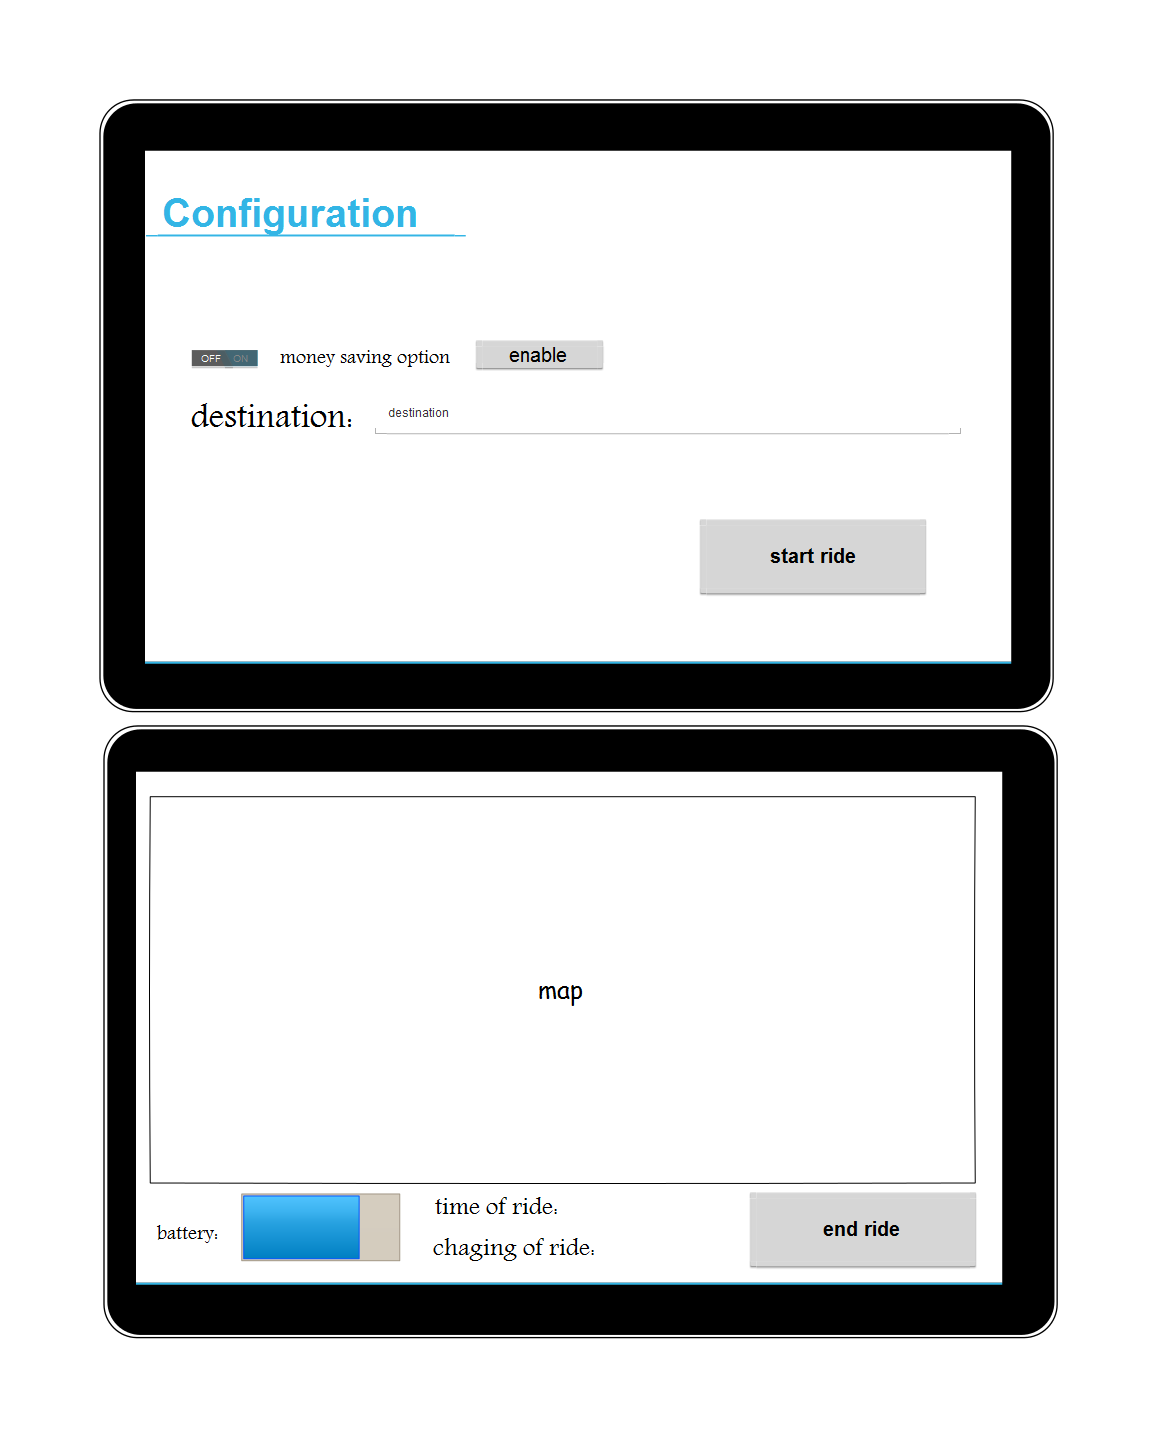
\includegraphics[scale=0.25]{Screen.png} 
	\end{figure}
	At the initial page of the screen, users can choose either to enable the money save option or not. For the former case, user will be notified a suggested destination. Users can use the button START RIDE to ignite the engine. The lower figure shows the corresponding information during the ride. There is also a button for users to end the ride.
	
	\newpage
	\section{REQUIREMENT TRACEABILITY}
	In this section, we are going to show a precise list of all the functional requirements and their corresponding mapping to components in the architecture.(for more detailed view of how these components contact with others and the interfaces of these components, please refer to the high level architecture and the component interface)
	\begin{itemize}
		\item\textbf{[G1]}Users can register to the system and get the password by providing credentials and payment information
		\newline - Guest Application Manager
		\newline - Database Manager
		\newline - User
		
		\item\textbf{[G2]}Registered users can log in by providing the correct credentials
		\newline - User Application Manager
		\newline - Database Manager
		\newline - User
		
		\item\textbf{[G3]}Registered users can find the locations of available cars within a certain distance from their current location or from a specified address
		\newline - User Application Manager
		\newline - Database Manager
		\newline - Car 
		\newline - Area
		
		\item\textbf{[G4]}Among the available cars in a certain geographical region, users must be able to reserve a single car for up to one hour before they pick it up.
		\newline - User Application Manager
		\newline - Database Manager
		\newline - User
		\newline - Car
		\newline - Reservation
		\newline - Google Map api
		
		\item\textbf{[G5]}If a car is not picked‐up within one hour from the reservation, the system tags the car as available again, and the reservation expires; the user pays a fee of 1 EUR.
		\newline - Car
		\newline - Reservation
		\newline - Database Manager
		\newline - Car Application Manager
		\newline - Bank system
		
		\item\textbf{[G6]}A user that reaches a reserved car must be able to tell the system she’s nearby, so the system unlocks the car and the user may enter.
		\newline - User Application Manager
		\newline - Database Manager
		\newline - Reservation
		\newline - Car
		\newline - Google Map api
		
		\item\textbf{[G7]}As soon as the engine ignites, the system starts charging the user for a given amount of money per minute; the user is notified of the current charges through a screen on the car.
		\newline - Car Application Manager
		\newline - Database Manager
		\newline - Ride
		\newline - Car
		
		\item\textbf{[G8]}The user is notified of the current charges through the screen on the car
		\newline - Car
		\newline - Ride
		\newline - Database
		\newline - Car Application Manager
		
		\item\textbf{[G9]}The system stops charging the user as soon as the car is parked in a safe area and the user exits the car; at this point, the system locks the car automatically.
		\newline - Car Application Manager 
		\newline - Database Manager
		\newline - Car
		\newline - Area
		\newline - Google Map api
		
		\item\textbf{[G10]}The users can know the locations of the safe areas
		\newline - User Application Manager
		\newline - Database Manager
		\newline - Area
		\newline - Google Map api
		
		\item\textbf{[G11]}If the system detects the user took at least two other passengers onto the car, the system applies a discount of 10\% on the last ride.
		\newline - Car Application Manger 
		\newline - Database Manager 
		\newline - Ride
		\newline - DiscountAndPunish
		
		\item\textbf{[G12]}If a car is left with no more than 50\% of the battery empty, the system applies a discount of 20\% on the last ride.
		\newline - Car Application Manger 
		\newline - Database Manager 
		\newline - Car
		\newline - Ride
		\newline - DiscountAndPunish
		
		\item\textbf{[G13]}If a car is left at special parking areas where they can be recharged and the user takes care of plugging the car into the power grid, the system applies a discount of 30\% on the last ride.
		\newline - Car Application Manger 
		\newline - Database Manager 
		\newline - Car
		\newline - Area
		\newline - Ride
		\newline - DiscountAndPunish
		\newline - Google Map api
		
		\item\textbf{[G14]}If a car is left at more than 3 KM from the nearest power grid station or with more than 80\% of the battery empty, the system charges 30\% more on the last ride to compensate for the cost required to re-charge the car on-site.
		\newline - Car Application Manager
		\newline - Database Manager
		\newline - Car 
		\newline - Area
		\newline - Ride
		\newline - DiscountAndPunish
		\newline - Google Map api
		
		\item\textbf{[G15]}If the user enables the money saving option, he/she can input his/her final destination and the system provides information about the station where to leave the car to get a discount. This station is determined to ensure a uniform distribution of cars in the city and depends both on the destination of the user and on the availability of power plugs at the selected station.
		\newline - User Application Manager
		\newline - Database Manager
		\newline - Car
		\newline - Area
		\newline - Reservation
		\newline - Google Map api
		
		
		
	\end{itemize}
	\newpage
	\section{EFFORT SPENT}
	29/11/2016 ZHOU YINAN 3h DD basic structure and introduction part\\
	30/11/2016 ZHOU YINAN 1h add parts of component interface\\
	2/12/2016 ZHOU YINAN 1h add component interface and diagram\\
	4/12/2016 ZHOU YINAN 2h architecture and design pattern\\
	4/12/2016 ZHAO KAIXIN 4h component view,high level architecture\\
	4/12/2016 ZHAN YUAN 3h add deployment view and part of runtime\\
	5/12/2016 ZHOU YINAN 1h architecture and pattern\\
	5/12/2016 ZHAN YUAN 2.5h add part of runtime view \\
	6/12/2016 ZHOU YINAN 1h document structure modified	\\
	6/12/2016 ZHAO KAIXIN 2h requirement traceability\\
	7/12/2016 ZHAO kAIXIN 1h requirement traceability\\
	7/12/2016 ZHAN YUAN   2h user interface design
	
	
	\newpage
	\section{REFERENCES}
	- RASD v1.0 \\
	-  Specification Document Assignments AA 2016-2017
	

\end{document}